\documentclass[11pt]{article}
\setlength{\oddsidemargin}{0in}
\setlength{\evensidemargin}{0in}
\setlength{\textwidth}{6.5in}
\setlength{\parindent}{0in}
\setlength{\parskip}{\baselineskip}
\usepackage{amsmath,amsfonts,amssymb}
\usepackage{enumitem}
\usepackage{graphicx}
\usepackage[]{algorithmicx}
\usepackage{comment}
\usepackage{tkz-berge}
\usetikzlibrary{positioning, automata}
\usepackage[utf8]{inputenc}
\usepackage{graphicx}

\usepackage{fancyhdr}
\pagestyle{fancy}
\setlength{\headsep}{36pt}

\usepackage{hyperref}



\newcommand{\makenonemptybox}[2]{%
%\par\nobreak\vspace{\ht\strutbox}\noindent
\item[]
\fbox{% added -2\fboxrule to specified width to avoid overfull hboxes
% and removed the -2\fboxsep from height specification (image not updated)
% because in MWE 2cm is should be height of contents excluding sep and frame
\parbox[c][#1][t]{\dimexpr\linewidth-2\fboxsep-2\fboxrule}{
  \hrule width \hsize height 0pt
  #2
 }%
}%
\par\vspace{\ht\strutbox}
}
\makeatother

\begin{document}
\definecolor {processblue}{cmyk}{0.96,0,0,0}
\lhead{{\bf CSCI 3104, Algorithms \\ Exam 2 -- S12} }
\rhead{Name: \fbox{\phantom{This is a really long name}} \\ ID: \fbox{\phantom{This is a student ID}} \\ {\bf Profs.\ Chen \& Grochow\\ Spring 2020, CU-Boulder}}
\renewcommand{\headrulewidth}{0.5pt}

\phantom{Test}

\begin{small}
\noindent \textbf{Instructions:} This quiz is open book and open note. You \textbf{may} post clarification questions to Piazza, with the understanding that you may not receive an answer in time and posting does count towards your time limit (30 min for 1x, 37.5 min for 1.5x, 45 min for 2x). Questions posted to Piazza \textbf{must be posted as PRIVATE QUESTIONS.} Other use of the internet, including searching for answers or posting to sites like Chegg, is strictly prohibited. Violations of these are grounds to receive a 0 on this quiz. Proofs should be written in \textbf{complete sentences.} \textbf{Show and justify all work to receive full credit.} 

\noindent \textbf{YOU MUST SIGN THE HONOR PLEDGE. Your quiz will otherwise not be graded.}  
\noindent \textbf{Honor Pledge:} On my honor, I have not used any outside resources (other than my notes and book), nor have I given any help to anyone completing this assignment. 

\noindent \textbf{Your Name:} \underline{\hskip 250pt}
\end{small} 

\hrulefill 


\pagebreak 

\noindent \textbf{Standard 12.} Consider the following graph $G$. 

\begin{center}
\noindent 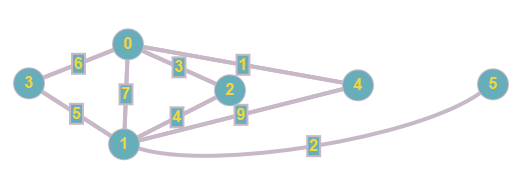
\includegraphics[scale=0.85]{S12_Graph.png}
\end{center}

\begin{enumerate}[label=(\alph*)]
\item Determine all the edges of $G$ which do not belong to any MST. Clearly justify your answer. \\

%YOUR ANSWER HERE

\pagebreak

\item Determine all edges of $G$ which belong to every MST. Clearly justify your answer. \\


%YOUR ANSWER HERE
\end{enumerate}

\end{document}


